The pacing problem is formalised as a finite Markov Decision Process  
\[
\langle \mathcal{S},\; \mathcal{A},\; \mathcal{P},\; r,\; \gamma \rangle,
\]
where  
\begin{itemize}
  \item \(\mathcal{S}\) is the state space, a tuple of seven components that capture the athlete’s physiological and contextual status.
  \item \(\mathcal{A}\) is the action set, consisting of three discrete commands: \emph{slow down}, \emph{keep going}, and \emph{accelerate}.
  \item \(\mathcal{P}(s'|s,a)\) is the transition dynamics, which describe how the state evolves given an action.
  \item \(r(s,a)\) is the reward function, which quantifies the desirability of each state–action pair.
  \item \(\gamma\) is the discount factor, controlling how future rewards are valued relative to immediate ones.
\end{itemize}

The MDP is implemented in the \texttt{RunnerEnv} class, which simulates the athlete's workout environment and decision-making process. The agent interacts with this environment by observing the current state, selecting an action, and receiving a reward while transitioning to a new state.

\begin{figure}[H]
\centering
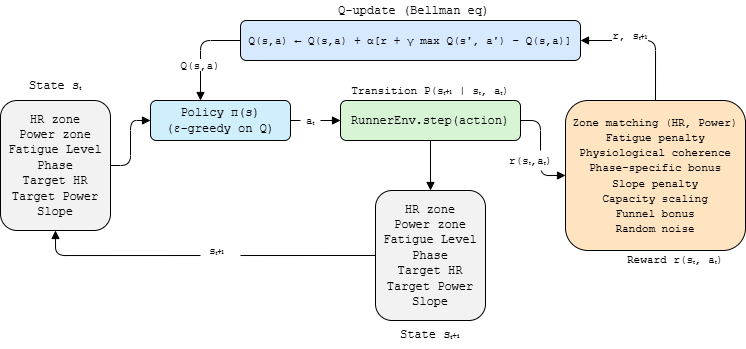
\includegraphics[width=0.99\textwidth]{images/draw_mdp.png}
\caption{Schema of the Markov Decision Process (MDP) for the pacing problem. The agent observes the current state \(s\), selects an action \(a\), and receives a reward \(r\) while transitioning to a new state \(s'\). The process is repeated, allowing the agent to learn an optimal policy over time.}
\label{fig:mdp_diagram}
\end{figure}

\subsection{State space \(\mathcal{S}\)}\label{subsec:state_space}
The states should encapsulate the athlete's physiological state in a specific moment, which is defined by the training program and the context of where the athlete is running. The components of the state space \(\mathcal{S}\) are summarised in Table~\ref{tab:state_space}.
\begin{table}[H]
\centering
\begin{tabular}{@{}lll@{}}
\toprule
\textbf{Component}        & \textbf{Meaning}                                        \\ \midrule
\verb|Heart Rate|         & Instantaneous heart-rate zone (Z1–Z5)                   \\
\verb|Power Zone|         & Instantaneous power zone (Z1–Z5)                        \\
\verb|Fatigue|            & Categorical fatigue (\emph{low/medium/high})            \\
\verb|Phase|              & Workout phase (warm-up, push, recover, cool-down)       \\
\verb|Target HR_zone|     & HR targets of current training segment                           \\ 
\verb|Target Power_zone|  & Power targets of current training segment                        \\
\verb|Slope|              & Terrain label (\emph{uphill/flat/downhill})             \\ \bottomrule
\end{tabular}
\caption{State space \(\mathcal{S}\) components.}
\label{tab:state_space}
\end{table}

\subsection{Action set \(\mathcal{A}\).}
The three admissible actions that an athlete can take during a workout are defined as:
\begin{itemize}
  \item \texttt{slow down} – reduce pace to lower heart rate and power.
  \item \texttt{keep going} – maintain current pace, allowing physiological drift.
  \item \texttt{accelerate} – increase pace to raise heart rate and power.
\end{itemize}

\subsection{Transition dynamics \(\mathcal{P}\)}
The most intricate component of the MDP is the definition of the state–transition kernel, i.e.\ how the athlete's physiological and contextual state evolves once an action is taken. In my simulation, this logic is encapsulated in \verb|RunnerEnv.step()|, which invokes four update routines every second, in the following order:

\begin{itemize}
  \item \verb|_update_power_zone(action)| – the chosen action (\emph{slow down}, \emph{keep going}, or \emph{accelerate}) instantaneously shifts the target wattage, and therefore the power zone. In real life, when you accelerate, your power output increases immediately; when you slow down, it drops right away.
  
  \item \verb|_update_hr_zone(action)| – this function updates the target heart rate zone based on the selected action. Unlike power, heart rate is a lagged variable: it does not change instantaneously, but drifts gradually toward the target zone. This models how the cardiovascular system responds over time.

  \item \verb|_update_fatigue(action)| – a dual-process model accumulates or dissipates fatigue depending on the heart rate, power zone, current workout phase, and the athlete's profile (elite, runner, or amateur).

  \item \verb|_advance_segment()| – the global time index is incremented, the active workout segment is updated accordingly, and the current slope level is recalculated from the GPX elevation trace.
\end{itemize}


Applied sequentially, these rules deterministically map the current pair \((s,a)\) to a unique next state \(s'\) at a granularity of 1 s; stochasticity is confined to the reward function, which injects small uniform noise to break ties.

\subsubsection{Reward function \(r(s,a)\)}
The reward function, together with the \verb|_update_fatigue(action)| routine (see~ \ref{subsubsec:fatigue}), forms the core of the simulator’s logic. These components determine how the agent is incentivised to follow the training plan while accounting for the athlete’s physiological state. The reward function is implemented in the \verb|compute_reward()| method of \verb|runner_env.py|, and outputs a scalar value that quantifies the agent’s performance in the current state and it's given by the sum of eight domain-specific terms:

\begin{itemize}
  
  \item \textbf{Zone–matching accuracy} - the absolute distance between the current and target HR / power zones is mapped to a piece-wise score \(\{+2.0,+0.5,-1.0,-2.5,-4.0\}\); HR and power contributions are then blended as \(0.4\,r_{\text{HR}} + 0.4\,r_{\text{Power}}\).

    \item \textbf{Fatigue management} – We maintain a continuous \verb|fatigue_score| \(f\in[0,10]\) whose dynamics are:
  \[
    \text{if phase}\in\{\text{recover},\text{cooldown}\}:\quad
      f \leftarrow \max\bigl(\mathrm{floor},\,f\,e^{-k}\;-\;d(f)\bigr),
  \]
  where
  \begin{itemize}
    \item \(k = 0.05 \times \text{fitness\_factor}\),
    \item \(d(f) = 0.1 \times \text{fitness\_factor}\times \sigma(f)\),
    \item \(\sigma(f) = 1/\bigl(1 + e^{-10\,(f-5)}\bigr)\),
    \item \(\mathrm{floor} = 0.1 \times \text{fitness\_factor}\).
  \end{itemize}
  In active phases (warm-up, push) \(f\) instead accumulates based on HR-zone gain constants, time in high zones, power coupling, FTP-scaling and session-type modifiers, then is clamped to \([0,10]\).  
  Finally, we classify \(f\) into \emph{low}/\emph{medium}/\emph{high} fatigue by comparing it against the 33rd and 67th percentiles of its own recent history, so that the medium/high labels adapt in real time to the athlete’s current strain.


  \item \textbf{Physiological coherence} – The agent computes \(\Delta_Z=\lvert Z_{\text{HR}}-Z_{\text{Power}}\rvert\). If \(\Delta_Z\) does not exceed the athlete-specific tolerance \(\{0.5,1.0,1.5\}\), a bonus of \(+1.0\) is awarded; otherwise a penalty \(-1.0\times(\Delta_Z-\text{tolerance})\) is applied.  This term encourages consistency between cardiovascular strain (HR zone) and mechanical output (power zone) without overpowering the other rewards.

  \item \textbf{Phase–action consistency} – This function reward the agent for taking actions that are consistent with the current phase of the workout.  For example, in the \emph{warm-up} phase, accelerating while still below the target HR is mildly encouraged \((+0.5)\), while braking is discouraged (-1); in the \emph{recover} phase, slowing down from supra-threshold HR receives +1 while accelerating is harshly penalised (-2).:

  \item \textbf{Terrain-aware pacing} – How the decision taken while the slope is changing can have different impact. Accelerating on an
        \emph{uphill} costs -2.0, braking on a \emph{downhill} -0.5; all other combinations are neutral.

  \item \textbf{Capacity scaling} –  The penalty for exceeding the athlete's \(Z_{\text{HR}}\) is attenuated by the efficiency factor (which is defined as \(\min(1,\text{FTP}/(6\,\text{kg}))\) ), so that lighter or fitter athletes are less penalised for visiting high zones as it should be in real-life.
  
  \item \textbf{Dynamic funnel bonus} – The funnel bonus is a dynamic reward that encourages the agent to maintain a precise pacing as the workout progresses.  It is defined as follows:
        \begin{itemize}
          \item During the first half of the workout, the agent receives +2.0 for entering the target zone and +0.5 for remaining inside.
          \item After halfway, the tolerance shrinks to \(\le 0\), meaning that entering the target zone gives +2.0 only once, while remaining inside yields +0.5.
        \end{itemize}
        This promotes sustained precision pacing.

    \item \textbf{Global fatigue decay \& stochasticity} – After summing all partial rewards, we multiply by 
    \[
      1-\min\!\bigl(\tfrac{f}{200},\,0.4\bigr)\,
    \]
    (capping the fatigue penalty at 40\%), and finally add uniform noise \(\mathcal{U}(-0.1,0.1)\) to break ties and mimic real‐world variability.

\end{itemize}

The final scalar is therefore
\[
r = 0.4\,r_{\text{HR}} + 0.4\,r_{\text{Power}}
     + 0.3\,r_{\mathrm{coh}} + 0.2\,r_{\mathrm{phase}}
     + r_{\mathrm{fatigue}} + r_{\mathrm{cap}}
     + r_{\mathrm{slope}} + r_{\mathrm{fun}},
\]
followed by the multiplicative decay and noise injection, as visible at the end of the \texttt{compute\_reward} method in \texttt{runner\_env.py}.


\subsubsection{Fatigue model}\label{subsubsec:fatigue}
The fatigue model implements a dual-process system: 

\begin{itemize}
    \item \textbf{Recovery/Cooldown Phases:} During these phases, fatigue dissipates through a combination of exponential and sigmoid decay, reflecting the natural recovery process. The decay rate and minimum fatigue floor are modulated by the athlete's fitness factor, ensuring that fitter athletes recover more efficiently. Constants are used to control the rate of decay and to prevent fatigue from dropping below a realistic minimum.
    \item \textbf{Warmup and Push Phases:} In active phases, fatigue accumulates based on the current heart rate (HR) and power zones. The accumulation rate is determined by zone-specific gain constants, which are further adjusted for the type of training session (e.g., interval, fartlek, endurance), the athlete's functional threshold power (FTP), and the time spent in high-intensity zones. Additional scaling is applied if both HR and power are in high zones, and a small random noise is introduced to simulate physiological variability.
    \item The resulting fatigue score is capped to \([0,10]\) and then discretized (low/medium/high) using real‐time percentiles of its history, ensuring the labels always reflect the athlete’s current relative fatigue.
\end{itemize}

